\section{DNS Query Analysis with Wireshark and \code{dig}}\label{sec:analysis}

% v1 source: Section 5 (methodology, response sections, SOA, NS, A, AAAA, TTL summary).
% Rules for this section (review feedback):
%   #3/#8  every screenshot is a labelled figure and is mentioned with \cref{fig:...}
%          next to the values it supports
%   #5     use the highlighted screenshots (see docs/action-plan notes)
%   #4     each table built from captures cites its source figure(s)
%   #2     RFC-defined behaviour (flags, EDNS, TTL, negative caching) carries a citation

\subsection{Methodology}\label{sec:methodology}

\subsection{Sections of a DNS response message}\label{sec:response-sections}

\subsection{SOA records}\label{sec:soa}

\subsection{NS records}\label{sec:ns}

\subsection{A records}\label{sec:a}

\subsection{AAAA records}\label{sec:aaaa}

\subsection{TTL summary by record}\label{sec:ttl}

% ------------------------------------------------------------
% SMOKE TEST: proves the shared ../figures, ../tables and the
% bibliography work. Delete this block when real content is in.
% ------------------------------------------------------------
\paragraph{Smoke test.}
The captured packets are shown in \cref{fig:capture-overview}; their TTL values are
summarized in \cref{tab:example} \parencite{rfc1035}.

\begin{figure}[htbp]
  \centering
  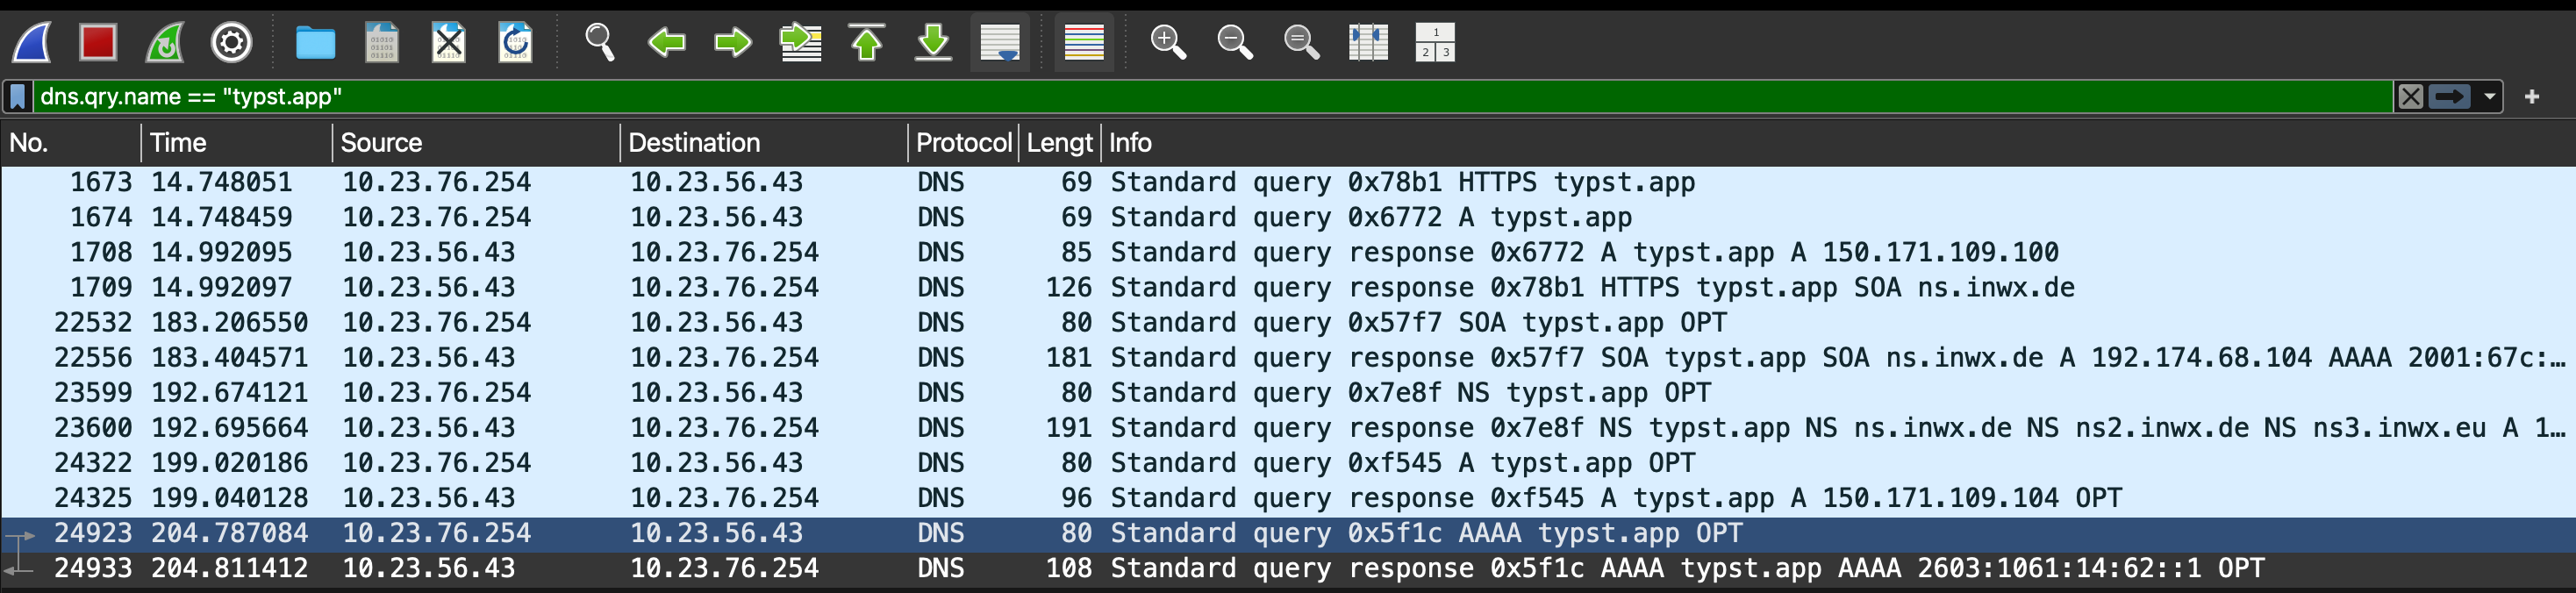
\includegraphics[width=\linewidth]{real dig typst.png}
  \caption{DNS packets for \code{typst.app} captured on Wi-Fi (\code{en0}) with the filter \code{dns.qry.name == "typst.app"}.}
  \label{fig:capture-overview}
\end{figure}

% Example shared table fragment. Include with % Example shared table fragment. Include with % Example shared table fragment. Include with \input{../tables/tab-example}
% (from docs/manuscript/vN/sections/*.tex).  Delete once real tables exist.
% Conventions: caption ABOVE (booktabs, no vertical rules), \label{tab:...},
% and a "Source" note naming the figure the values come from.
\begin{table}[htbp]
  \centering
  \caption{Observed TTL for each record type in \code{typst.app} (example fragment).}
  \label{tab:example}
  \begin{tabular}{@{}llr@{}}
    \toprule
    Type & Name & TTL (s) \\
    \midrule
    NS   & \code{typst.app.} & 4076 \\
    A    & \code{typst.app.} & 300  \\
    \bottomrule
  \end{tabular}

  \smallskip
  \footnotesize Source: \cref{fig:capture-overview}.
\end{table}

% (from docs/manuscript/vN/sections/*.tex).  Delete once real tables exist.
% Conventions: caption ABOVE (booktabs, no vertical rules), \label{tab:...},
% and a "Source" note naming the figure the values come from.
\begin{table}[htbp]
  \centering
  \caption{Observed TTL for each record type in \code{typst.app} (example fragment).}
  \label{tab:example}
  \begin{tabular}{@{}llr@{}}
    \toprule
    Type & Name & TTL (s) \\
    \midrule
    NS   & \code{typst.app.} & 4076 \\
    A    & \code{typst.app.} & 300  \\
    \bottomrule
  \end{tabular}

  \smallskip
  \footnotesize Source: \cref{fig:capture-overview}.
\end{table}

% (from docs/manuscript/vN/sections/*.tex).  Delete once real tables exist.
% Conventions: caption ABOVE (booktabs, no vertical rules), \label{tab:...},
% and a "Source" note naming the figure the values come from.
\begin{table}[htbp]
  \centering
  \caption{Observed TTL for each record type in \code{typst.app} (example fragment).}
  \label{tab:example}
  \begin{tabular}{@{}llr@{}}
    \toprule
    Type & Name & TTL (s) \\
    \midrule
    NS   & \code{typst.app.} & 4076 \\
    A    & \code{typst.app.} & 300  \\
    \bottomrule
  \end{tabular}

  \smallskip
  \footnotesize Source: \cref{fig:capture-overview}.
\end{table}

